\documentclass[reqno, 11pt, final]{article}
\usepackage[margin=1in]{geometry} % Margin size, enclosed in [ ] (NOT { })
\geometry{letterpaper} % Paper size
\usepackage{graphicx}
\usepackage{amssymb}
\usepackage{amsfonts}
\usepackage{amsmath}
\usepackage[retainorgcmds]{IEEEtrantools}
\usepackage{epstopdf}
\usepackage{fullpage}
\usepackage{wrapfig}
\usepackage{textcomp}
\pagestyle{plain}

\usepackage[small,bf]{caption} %Sets caption text to SMALL and BOLDFACED
\setlength{\parindent}{0in} % Sets paragraph indent size (tab length)
\setlength{\footskip}{0.5in}
\DeclareGraphicsRule{.tif}{png}{.png}{`convert #1 `dirname #1 `/`basename #1 .tif` .png}

\newcommand{\bolditalic}[1]{\textbf{\textit{#1}}}
\newcommand{\tuple}[1]{\begin{pmatrix} #1 \end{pmatrix}}
\newcommand{\bbmatrix}[1]{\begin{bmatrix} #1 \end{bmatrix}}
\newcommand{\intd}{\, \mathrm{d}}
\newcommand{\R}{\mathbb{R}}
\newcommand{\Q}{\mathbb{Q}}
\newcommand{\N}{\mathbb{N}}
\newcommand{\C}{\mathbb{C}}
\newcommand{\Z}{\mathbb{Z}}
\newcommand{\tab}{\hspace{0.5in}}
\newcommand{\textfahrenheit}{\textdegree{}F}

\begin{document}
\begin{flushright}
Charlie Jiang \\
October 7, 2014
\\[12pt]
\end{flushright}

\textbf{Stanford Solar Car Project | Analyzing Charging Configurations for Sunwhale} \\
\renewcommand{\baselinestretch}{1.1} % Line spacing = 1.1x

\section{Fitting Concentrators Above Car in Bounding Box}

We will orient ourselves so that we are looking at the bounding box from its smallest face, standing upright. So the box is $1.8$ m horizontally and $2.2$ m vertically. \\

Here, the basic assumption is that the array (whether with a monocoque or a topshell) is placed facing the sun into the bottom left corner of the box (in the given orientation), and rows of concentrators are placed at the top of the bounding box such that no part of the array or concentrators are shaded. \\

We will consider two cases, a monocoque and topshell. The difference is that for the topshell case, the array is separate from the car body, so we will have to account for the car body placed somewhere in the bounding box. We will ignore the canopy in both cases, assuming it can fit within the box in a non-intrusive way.

\subsection{Monocoque}

\begin{figure}[h]
	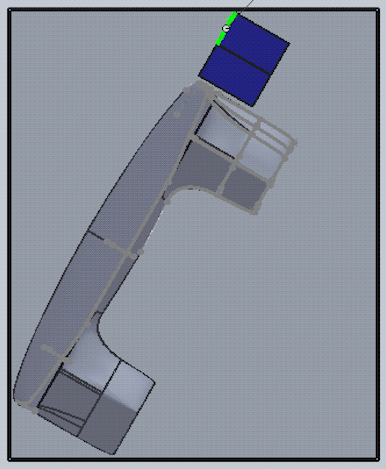
\includegraphics[scale=0.5]{charging_configs_fittingconcentratorsCADEx}
	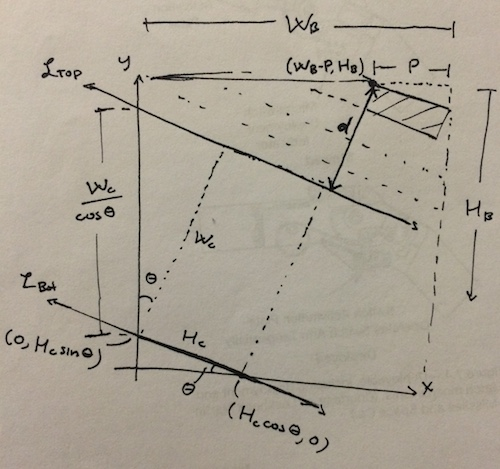
\includegraphics[scale=0.5]{charging_configs_fittingconcentratorsschematic}
	\caption{(Left) Example CAD of charging configuration with monocoque. (Right) Diagram of ideal monocoque and concentrator placement within bounding box}
\end{figure}

We treat the car as a rectangle with width $W_c$ and height (i.e. length of fairing + side of body) $H_c$. The car (and concentrators) is tilted at an angle $\theta$ from vertical to directly face the sun. At this angle, the car is placed into the bottom left corner of the box, which we will consider the origin of a Cartesian plane. $L_{BOT}$ and $L_{TOP}$ are lines that we can extend from the shorter sides of the car rectangle. \\

In order for the concentrators to face the sun with minimal shading, they must be oriented at angle $\theta$ entirely on top of one another. The range of positions for the concentrators to maximize their number is anywhere between the dashed lines parallel to $L_{TOP}$. To maximize the number of concentrators (which we will treat as rectangles with width $w$ and length $l$), the topmost one must fit as well as possible in the bounding box's upper right corner. \\ 

The number of rows of concentrators depends, then, on $d,$ the distance from the point at which the topmost concentrators meets the top of the bounding box, to the line $L_{TOP}.$ Now, to calculate $d$. \\

The equation of $L_{TOP}$, as can be determined from the diagram, is
	\[ L_{top}(x) = -\tan(\theta) \cdot x + H_c \sin \theta + \frac{W_c}{\cos \theta}. \]
The point of interest has coordinates $(W_B - P, H_B),$ where $P = l \cos \theta.$ Then
	\[ d = \frac{\big| \tan\theta \cdot (W_B-P) + H_B - H_C \sin \theta - W_C / \cos \theta \big|}{\sqrt{\tan^2 \theta + 1}}. \]
Noting that the denominator is merely $\sec\theta = 1/\cos\theta,$ and subsituting for $P$, we end with
	\begin{align*} d
		& = \cos\theta \cdot \Big( \tan\theta \cdot (W_B-l\cos\theta) + H_B - H_C \sin \theta - \frac{W_C}{\cos \theta} \Big) \\
		& = W_B\sin\theta - l\cos\theta\sin\theta + H_B\cos\theta - H_C\sin\theta\cos\theta - W_C \\
		& = W_B\sin\theta + H_B\cos\theta - \big(\frac{H_C+l}{2}\big) \sin2\theta - W_C. \end{align*}
The number of rows of concentrators that can fit, then, is
	\[ N_{rows} = \text{floor}(d/w), \]
where $w$ is the width of a concentrator element. \\

We can now determine the number of rows of concentrators that can fit as a function of the angle $\theta$ for our case, where we have
	\[ W_B = W_C = 1.8 \text{m}, \; H_B = 2.2 \text{m}, \; H_C \approx 0.55 \text{m}, \; l = 12 \text{in} = 0.30 \text{m} \]
(the value of $H_C$ is based on the height of Sunwhale-025; the value of $l$ is estimated from the concentrator focal length plus room for enclosure mechanisms). \\

\subsection{Topshell}

The primary differences between a topshell/bottomshell configuration, and a monocoque one, are:
\begin{enumerate}
	\item The topshell takes up a smaller ``rectangle'' than the full car (i.e., $W_C$ and $H_C$ can be smaller).
	\item The rest of the car must be accounted for in the bounding box.
\end{enumerate}
The latter, as far as I can tell, will not actually have an effect on our calculation from above. Let us suppose that the car body will be placed vertically at one edge of the bounding box, leaving space for the topshell to be arranged as shown:

\begin{figure}[h]
	\centering 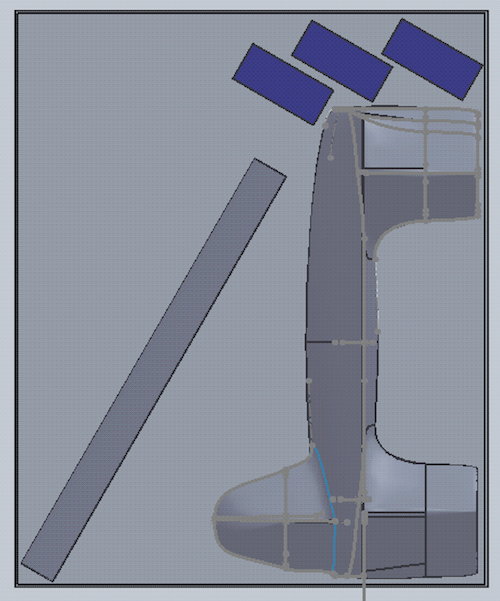
\includegraphics[scale=0.5]{charging_configs_fittopshellschematic}
	\caption{Possible topshell/bottomshell charging configuration.}
\end{figure}

The concentrator elements have $l \approx 0.3 m,$ so they can easily fit in the bounding box above the car body at any angle from $0-30^{\circ}$. Other rows of concentrators can fit in line, horizontally, as shown. The car body does not take up enough space horizontally in the bounding box to worry about concentrators not fitting horizontally either. \\

Thus, we only need consider various topshell sizes, i.e. altering $W_C$ and $H_C$ in our calculations.

\newpage
\section{Performance vs. Number of Concentrators}

\end{document}